\section{Técnicas de filtrado de ruido en señales de habla}

\subsection{Ruidos estacionarios y no-estacionarios}

Los filtros de ruidos en señales de habla los podemos dividir en dos grupos. Por un lado, tenemos los filtros que permiten suprimir ruidos estacionarios y por otro lado, los que logran filtrar tanto ruido estacionario como no-estacionario.

Los filtros de ruidos estacionarios en señales de habla, en general, trabajan de la siguiente manera:

\begin{enumerate}
	\item Detectan períodos de no-habla.
	\item En el período de no-habla, estiman la magnitud del espectro del ruido.
	\item A la magnitud del espectro de la señal de habla ruidosa, le restan una estimación de la magnitud del espectro del ruido.
	\item Utilizando la fase de la señal ruidosa y la magnitud obtenida en el paso anterior, construyen la señal de habla filtrada.
\end{enumerate}

Este proceso tiene un inconveniente evidente. Para lograr un filtrado exitoso se requiere que el ruido no cambie durante los períodos de habla, es decir solo logra filtrar ruidos estacionarios.

Los ruidos no-estacionarios se caracterizan por ser de aparición espontánea, no periódica y usualmente de corta duración, haciendo sumamente compleja su correcta caracterización por medio de modelos matemáticos.

En las siguientes secciones veremos un repaso de las técnicas de filtrado de ruido estacionario y no-estacionario en señales de habla.

\subsection{Técnicas tradicionales de filtrado de ruido en señales de habla}

En la presente sección repasaremos algunas de las técnicas de filtrado comúnmente utilizadas para suprimir ruidos en señales de habla.

\subsubsection{Sustracción espectral}
\label{sec:sustraccion_espectral}

La técnica conocida como sustracción espectral, en su versión más básica, consiste en sustraer del espectro de la señal ruidosa una estimación del espectro del ruido obtenido en periodos de no habla.

Formalmente, dada la señal de habla ruidosa $y(n)$, la señal de habla sin ruido $x(n)$ y el ruido aditivo $d(n)$ tenemos que:

\begin{equation*}
	y(n) = x(n) + d(n)
\end{equation*}

Tomando la DFT de ambos lados:

\begin{equation*}
	Y(\omega) = X(\omega) + D(\omega)
\end{equation*}

y por lo tanto:

\begin{equation*}
	X(\omega) = Y(\omega) - D(\omega)
\end{equation*}

lo cual se puede descomponer en:

\begin{equation*}
	|X(\omega)| = |Y(\omega) - D(\omega)| \qquad \text{y} \qquad \phi_{X(\omega)} = \phi_{Y(\omega) - D(\omega)}
\end{equation*}

Suponiendo que la fase de $Y(\omega)$ es aproximadamente colineal a la fase de $D(\omega)$ se obtiene que:

\begin{equation*}
	|\hat{X}(\omega)| = |Y(\omega)| - |D(\omega)| \qquad \text{y} \qquad \hat{\phi}_{X(\omega)} = \phi_{Y(\omega)}
\end{equation*}

Donde la magnitud de la señal de ruido $D(\omega)$ se estima en los periodos de no-habla.

Un problema evidente que surge a partir de las aproximaciones realizadas, es que la resta $|Y(\omega)| - |D(\omega)|$ puede llevar a un valor negativo de $|\hat{X}(\omega)|$. En la práctica usualmente lo que se hace es implementar un rectificador de media onda, es decir:

\begin{equation*}
	|\hat{X}(\omega)| = \begin{cases} 
		|Y(\omega)| - |D(\omega)| & \text{si} \quad |Y(\omega)| >  |\hat{D}(\omega)| \\
		0 & \text{si} \quad |Y(\omega)| \leq  |\hat{D}(\omega)|\\
	\end{cases}
\end{equation*}

La señal de habla mejorada se obtiene simplemente tomando la iDFT, es decir:

\begin{equation*}
	\hat{x}(n) = iDFT \left\{ |\hat{X}(\omega)| e^{\phi_{Y(\omega)}} \right\}
\end{equation*}

La no linealidad introducida por el rectificador generan, en el dominio del tiempo, unos picos que son perceptibles para el oído humano, a dicho ruido se lo conoce como ruido musical. En ocasiones este ruido introducido por la sustracción espectral puede resultar en un sonido incluso más desagradable que el generado por el ruido aditivo.

Por lo tanto, el método de sustracción espectral es relativamente sencillo de implementar, pero trae principalmente dos problemas:

\begin{enumerate}
	\item El ruido musical generado por el rectificador de media onda.
	\item La necesidad de contar con pausas en la señal de habla para una correcta estimación de $|D(\omega)|$.
\end{enumerate}

Si bien existen técnicas para combatir los problemas (1) y (2) \cite{speech_enhancement_theory_and_practice}, los sistemas resultantes terminan siendo complejos de llevar a la práctica.

\subsubsection{Filtro de Wiener}

El método de sustracción espectral aprovecha la característica aditiva del ruido para obtener la señal de habla filtrada por medio de restar una estimación de la magnitud del ruido. Este método, si bien es efectivo, resulta no ser óptimo en el sentido del error cuadrático medio. 

El filtro de Wiener, aplicado al filtrado de ruidos en señales de habla, permite obtener un filtro óptimo utilizando el criterio del error cuadrático medio. 

Dada una señal objetivo $d(n)$, la señal a filtrar $y(n)$ y el siguiente sistema:


\begin{figure}[H]
	\centering
	\centerline{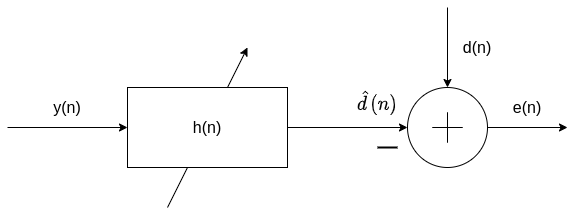
\includegraphics[scale=0.6]{images/ch3/wiener.png}}
	\caption{Filtro de Wiener.}
	\label{fig:ch3_wiener_filter}
\end{figure}


El filtro óptimo, en el sentido del error cuadrático medio, viene dado por:

\begin{equation*}
	h_{opt} = R_{yy}^{-1} R_{dy}
\end{equation*}

\noindent donde $R_{yy}$ es la matriz de autocorrelación del proceso $y$, y $ R_{dy}$ es el vector de correlación cruzada entre el proceso $y$ y la variable aleatoria $d$.

Por otro lado, si consideramos, nuevamente un ruido aditivo:

\begin{equation*}
	y(n) = x(n) + n(n)
\end{equation*}

\noindent tendremos que el filtro óptimo viene dado por \cite{speech_enhancement_theory_and_practice}:

\begin{equation*}
	h_{opt} = \left( R_{xx} + R_{nn} \right)^{-1} R_{xx}
\end{equation*}

\noindent o en el dominio de la frecuencia \cite{speech_enhancement_theory_and_practice}:

\begin{equation*}
	H(\omega) = \frac{P_{xx}(\omega)}{P_{xx}(\omega) + P_{nn}(\omega)}
\end{equation*}

\noindent donde P es la densidad espectral de potencia. Dado

\begin{equation*}
	X(\omega) = DTFT\{ x_{(n)} \} \qquad \text{y} \qquad N(\omega) = DTFT\{ n_{(n)} \}
\end{equation*}

\noindent entonces, la densidad espectral de potencia viene dada por \cite{intuitive_probability_and_random_processes_using_matlab}:

\begin{equation*}
	P_{xx} = E[ | X(\omega) |^2 ] \qquad \text{y} \qquad P_{nn} = E[ | N(\omega) |^2 ]
\end{equation*}

Conocido ya el filtro óptimo en el sentido del error cuadrático medio, el siguiente problema a resolver es la estimación de las densidades $P_{xx}$ y $P_{nn}$ o las respectivas funciones de auto-correlaciones.

Una de las técnicas utilizadas en la práctica consiste en modelar la señal de habla como la respuesta de un sistema LTI, como el que se muestra en la figura \ref{fig:ch3_voice_modeling} \cite{spoken_language_processing}. 

Los sonidos del tipo vocálicos son modelados con una excitación periódica y los del tipo no-vocálicos modelados con una excitación aleatoria. El sistema LTI modela el tracto vocal y a la salida del sistema se obtiene la señal de habla.

\begin{figure}
	\centering
	\centerline{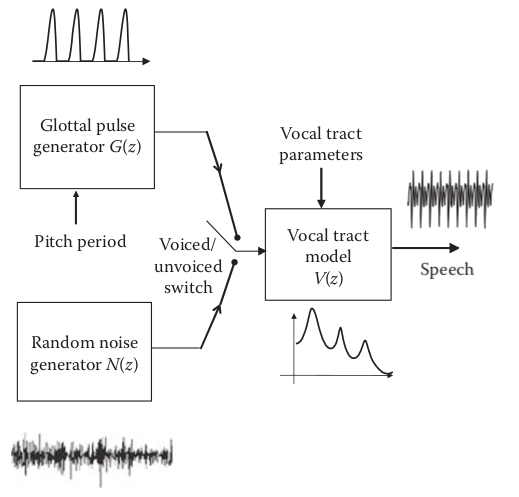
\includegraphics[scale=0.5]{images/ch3/voice-modeling.png}}
	\caption{Modelo de las señales de habla. Imagen tomada de \cite{speech_enhancement_theory_and_practice}.}
	\label{fig:ch3_voice_modeling}
\end{figure}


Al tracto vocal usualmente se lo modela como un sistema formado únicamente por polos \cite{spoken_language_processing}, con lo que $V(z)$ tiene una transformada Z de la forma:

\begin{equation*}
	V(z) = \frac{q}{1 - \sum_{k=1}^{p} a_k z^{-k}}
\end{equation*}

Por lo tanto, en el dominio del tiempo, la señal de habla responde a la ecuación diferencial:

\begin{equation*}
	x(n) = \sum_{k=1}^{p}a_k x(n-k) + g \; u(n)
\end{equation*}

\noindent donde $u(n)$ representa la excitación.

Estimados los coeficientes $a_k$ se podría obtener la densidad espectral de potencia $P_{xx}$ y con ello obtener el filtro óptimo. En \cite{all_pole_modeling_of_degraded_speech} utilizan la técnica de máximo a posteriori para estimar los coeficientes $a_k$

A diferencia de la sustracción espectral, en este caso no fue necesario utilizar los momentos de pausa para estimar la magnitud del espectro del ruido, pero si se requirió la utilización de modelos para la señal de voz y modelos para el ruido aditivo. 

En algunos casos de usos se puede obtener un filtro de ruidos en señales de habla con un buen desempeño, pero cuando las condiciones reales se alejan del modelo, el sistema comienza a fallar, lo que sucede especialmente con el modelo del ruido.

\subsection{Técnicas de filtrado de ruido en señales de habla basadas en filtros adaptativos}
\label{sec:adaptive_filter}

\subsubsection{Arquitectura de un filtro adaptativo como cancelador de ruido}
\label{sec:adaptive_filter_architecture}

En algunas aplicaciones resulta posible la utilización de más de un micrófono para captar las señales de habla. En estos casos resulta posible la utilización de un filtro adaptativo \cite{fundamentals_of_adaptive_filtering}.

Usualmente en este tipo de situaciones se tiene un micrófono, el cual capta la señal de habla más el ruido aditivo y por otro lado, un micrófono que capta únicamente el ruido.

A continuación podemos ver la configuración de un cancelador de ruido basado en un filtro adaptativo:

\begin{figure}[H]
	\centering
	\centerline{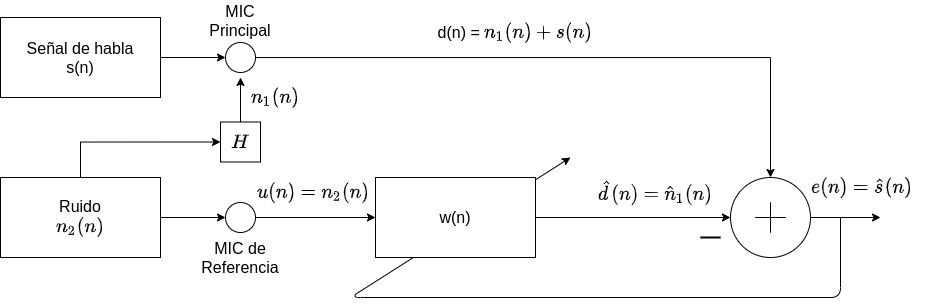
\includegraphics[scale=0.5]{images/ch3/af-se-setup.png}}
	\caption{Filtro adaptativo configurado como cancelador de ruido. Imágen tomada de \cite{a_family_of_adaptive_filter_slgorithms_in_noise_cancellation_for_speech_enhancement}.}
	\label{fig:ch3_af-se-setup}
\end{figure}

El micrófono principal captura la señal de habla $s(n)$ corrompida por el ruido $n_1(n)$ . Por otro lado, el micrófono de referencia captura la señal de ruido $n_2(n)$, el cual está correlacionado con el ruido $n_1(n)$. 

El ruido $n_2(n)$ pasa por el filtro adaptativo, el cual lo transforma para obtener una estimación del ruido $n_1(n)$. Al restar la señal de habla ruidosa, con una estimación del ruido que la corrompió originalmente, es posible obtener una estimación de la señal de habla. 

Este modelo supone que existe un filtro $H$, el cual transforma el ruido $n_2(n)$ en $n_1(n)$. Dada la configuración de la figura \ref{fig:ch3_af-se-setup}, el filtro adaptativo tratará de estimar los coeficientes del filtro $H$. El buen desempeño del filtro estará principalmente dado por la exactitud con la que logre aproximar a $H$.

El filtro se auto-ajusta continuamente, de manera tal que se minimice el error cuadrático medio entre $n_1(n)$ y $\hat{n}_1(n)$ . La señal de error viene dada por:

\begin{equation*}
	e(n) = \hat{s}(n) = n_1(n) + s(n) - \hat{n}_1(n)
\end{equation*}

\noindent calculando el valor esperando de ambos lados:

\begin{align*}
	\mathbb{E}[e^2] &= \mathbb{E}[( n_1 + s - \hat{n}_1)^2] \\ \\
	&= \mathbb{E}[n_1^2 + s^2 + \hat{n}_1^2 - 2 n_1 s - 2 \hat{n}_1 n1]
\end{align*}

Si la señal de habla se encuentra descorrelacionada con los ruidos $n_1$ y $n_2$, y además ambos ruidos están correlacionados entre sí, es decir:

\begin{equation*}
	\mathbb{E}[n_1 s] = 0 \qquad \mathbb{E}[n_2 s] = \mathbb{E}[\hat{n}_1 s] = 0 \qquad \mathbb{E}[n_1 n_2] \neq 0
\end{equation*}

\noindent obtenemos que:

\begin{align*}
	\mathbb{E}[e^2] = \mathbb{E}[s^2] + \mathbb{E}[(n_1 - \hat{n}_1)^2]
\end{align*}

Por lo que el filtro, al minimizar $\mathbb{E}[( n_1 + s - \hat{n}_1)^2]$, también minimiza $\mathbb{E}[(n_1 - \hat{n}_1)^2]$.


\subsubsection{Filtro RLS}
\label{sec:adaptive_filter_rls}

En la sección anterior vimos la arquitectura de un filtro adaptativo utilizado para filtrar ruidos en señales de habla. Además de definir la configuración del filtro es necesario establecer la regla de optimización. Alguno de los algoritmos mas comúnmente utilizados son \cite{a_family_of_adaptive_filter_slgorithms_in_noise_cancellation_for_speech_enhancement}; el LMS, el NLMS, el RLS y el APA.

En \cite{a_family_of_adaptive_filter_slgorithms_in_noise_cancellation_for_speech_enhancement} podemos ver que, entre los algoritmos evaluados, el RLS es el que logra el menor error cuadrático medio y el que tiene mayor velocidad de convergencia. En base a estos resultados se decidió limitar el presente trabajo a la utilización del algoritmo RLS. 

El algoritmo RLS describe la solución recursiva al problema de cuadrados mínimos ponderado y regularizado definido por \cite{fundamentals_of_adaptive_filtering}:

\begin{equation*}
	\min_{ \omega} \left[\lambda^{N+1} \omega^* \Pi \omega + \sum_{j=0}^N \lambda^{N-j} |d(j) - u_j \omega |^2 \right]
\end{equation*}

\noindent donde $ 0 \ll \lambda \leq 1$ es el factor de olvido, el cual selecciona qué tanta importancia se le debe dar a las muestras pasadas. 

Desde el punto de vista de los filtros adaptativos, el algoritmo RLS surge a partir de aproximar las matrices de autocorrelación de los procesos $d$ y $u$ para lograr aproximar el gradiente de la función de costo $J(\omega) = \mathbb{E} | d - u \omega |^2$.

El filtro óptimo viene dado por medio de la ecuación de Wiener:

\begin{equation*}
	w^o = R_u^{-1}R_{du}
\end{equation*}

Utilizando la técnica de gradiente descendiente se obtiene la recursión:

\begin{equation*}
	w_i = w_{i-1} - \mu(i) \left[ \nabla^2_\omega J(\omega_{i-1}) \right] \left[ \nabla_w J(w_{i-1}) \right]^*
\end{equation*}

\noindent la cual puede reducirse a \cite{fundamentals_of_adaptive_filtering}:

\begin{equation*}
	w_i = w_{i-1} + \mu(i) (\epsilon(i) I + R_{uu} )^{-1} \left( R_{du} - R_{uu} w_{i-1} \right)
\end{equation*}

Como en la práctica no se suele conocer las matrices de autocorrelación $R_u$ y $R_{du}$, éstas son aproximadas. Para el caso del filtro RLS las aproximaciones utilizadas vienen dadas por:

\begin{equation*}
	\hat{R}_{du} = u_i^* d(i) \qquad \text{y} \qquad \hat{R}_{uu} = \frac{1}{i+1} \sum_{j=0}^{i} \lambda^{i-j} u_j^* u_j
\end{equation*}

Para $R_u$ se está usando el estimador de media muestral incluyendo el factor de olvido $\lambda$ y para $\hat{R}_{du}$ se están utilizando los valores instantáneos.

\subsubsection{Error en estado estacionario}
\label{sec:adaptive_filter_stationary_error}

Como vimos en la sección anterior, los filtros adaptativos buscan minimizar la función de costo $J(\omega) = \mathbb{E} | d - u \omega |^2$. La solución óptima en el sentido del error cuadrático medio es \cite{fundamentals_of_adaptive_filtering}:

\begin{equation*}
	w^o = R_u^{-1}R_{du}
\end{equation*}

Entonces el mínimo error vendrá dado por $J(w_o)$, el cual se puede probar que es \cite{fundamentals_of_adaptive_filtering}:

\begin{equation*}
	J_{min} = J(w_o) = \sigma_d^2 - R_{ud} R_{u}^{-1} R_{du}
\end{equation*}

Es decir, en el caso de tener caracterizados los procesos estocásticos y contar con la matrices de autocorrelación, el error de aproximación de la señal $d(n)$ será mayor o igual a $J_{min}$. Para el caso donde no se cuenta con estas matrices y se recurra a aproximaciones como en el algoritmo RLS, el error va a ser aún mayor, ya que las aproximaciones estocásticas introducen ruido en la estimación del gradiente \cite{fundamentals_of_adaptive_filtering}.

\subsubsection{Procesamiento de las señales de habla}
\label{sec:filtro_adaptativo_procesamiento_de_señales}

Los filtros adaptativos trabajan de forma recursiva, es decir, para obtener la salida en el tiempo $n$ se necesita el estado del filtro en el tiempo $n-1$ y las señales $d(n)$ y $u(n)$. 

Utilizando las aproximaciones de $R_u$ y $R_{du}$ vistas en la sección anterior y definiendo:

\begin{equation*}
	\mu(i) = \frac{1}{i+1} \qquad \text{y} \qquad \epsilon(i) = \frac{\lambda^(i+1) \epsilon}{i + 1}
\end{equation*}

se puede obtener la siguiente recursión \cite{fundamentals_of_adaptive_filtering}:

\begin{equation*}
	w_i = w_{i-1} + P_i u_i^* \left( d(i) - u_i w_{i-1} \right)
\end{equation*}

donde:

\begin{equation*}
	P_i = \lambda^{-1} \left(P_{i-1} - \frac{\lambda^{-1} P_{i-1} u_i^* u_i P_{i-1}}{1 + \lambda^{-1} u_i P_{i-1} u_i^*} \right)
\end{equation*}

con la condición inicial $P_{-1}=\epsilon^{-1}$ y $ 0 \ll \lambda \le 1$.

El procesamiento de una señal de habla consiste en los siguientes pasos:

\begin{enumerate}
	\item Inicializar los coeficientes del filtro.
	\item Usando $d(i)$ y $u(i)$, obtener $P_i$ y $w_i$.
	\item Obtener la señal de habla filtrada dada por la señal $e(i) = d(i) - u_i w_i $.
	\item Volver al paso 2.
\end{enumerate}

\subsection{Técnicas de filtrado de ruido en señales de habla basadas en redes neuronales}
\label{sec:tecnicas_filtrado_redes_neuronales}

La limitante que poseen los filtros adaptativos es la necesidad de contar con una señal de referencia, lo cual conlleva a la necesidad de utilizar múltiples micrófonos. En algunos casos de usos, tal requerimiento es incluso prohibitivo lo cual impulsa la búsqueda de nuevas soluciones. 

Como vimos en la sección \ref{sec:sustraccion_espectral}, una técnica comúnmente utilizada para filtrar señales de habla corrompidas por ruido, es la técnica de sustracción espectral. Esta técnica, consiste en obtener una estimación del espectro del ruido durante los periodos de silencio. El espectro estimado se usa para filtrar la señal de habla corrompida. Una desventaja de esta técnica es que si el ruido es no-estacionario, la variabilidad del mismo no permite mantener una correcta estimación del espectro del ruido.

En la última década, el gran avance que hubo en el desarrollo de redes neuronales \cite{deep_learning} permitió elaborar redes capaces de filtrar señales de habla corrompidas incluso en casos de uso donde solo se cuenta con la información provista por un solo micrófono. 

A diferencia de la sustracción espectral o de los filtros adaptativos que se basan en la utilización de técnicas de procesamiento de señales, el filtro basado en redes neuronales es una técnica basada en datos. Es decir, para poder desarrollar estos filtros se necesitan de una gran cantidad de señales corrompidas que permitan entrenar la red de manera que los parámetros de la misma se ajusten de forma tal que se minimice la diferencia entre las señales filtradas y las señales de habla sin ruido.

\subsubsection{Información de entrada y de salida}

Se ha demostrado que el tipo de información que resulta más relevante para entrenar este tipo de redes, es la potencia espectral logarítmica \cite{a_regression_approach_to_speech_enhancement_based_on_deep_neural_networks}. 

Haciendo una simplificación, podemos pensar que como entrada de la red, se usa el espectro de la señal corrompida por ruido y a la salida, como señal objetivo, se usa el espectro de la señal original, de manera que la red aprenda a realizar las transformaciones necesarias para llegar de una señal a la otra.

Dado que las señales de habla ruidosas son no-estacionarias es necesario analizarlas por tramos, por tal motivo resulta conveniente la utilización de la transformada de Fourier de tiempo corto STFT. 

Dada la señal de habla ruidosa $d[n]$, la información utilizada para entrenar la red es:

\begin{equation*}
	X(n, w) = log(|STFT\{d[n]\}|^2) = log(|D(n, w)|^2)
\end{equation*}

Por otro lado la señal objetivo sera $s[n]$, por lo tanto la información utilizada a la salida será:

\begin{equation*}
	Y(n, w) = log(|STFT\{s[n]\}|^2) = log(|S(n, w)|^2)
\end{equation*}

Dado que se requiere construir un filtro de ruido para aplicaciones de tiempo real, resulta necesario obtener $Y(n, w)$ usando únicamente la señal de habla ruidosa hasta el tiempo $n$, es decir $\{..., X(n - 2, w), X(n - 1, w), X(n, w)\}$. 

Hay otras aplicaciones que no requieren un procesamiento en tiempo real de la señal de habla, donde para obtener $Y(n, w)$ se podría utilizar tanto información pasada como información futura. Por ejemplo, una aplicación de separación de habla se encarga de tomar una señal de audio mezclada y separarla en las distintas fuentes que la produjeron. Esta aplicación no requiere que se realice el procesamiento en tiempo real. Para obtener $Y(n, w)$ se puede usar tanto información pasada $\{..., X(n - 2, w), X(n - 1, w), X(n, w)\}$ como futura $\{X(n +1, w), X(n + 2, w), ...\}$. 

Usualmente se trabajan con 3 tipos de estructuras de redes en las aplicaciones de cancelación de ruido en señales de habla \cite{a_regression_approach_to_speech_enhancement_based_on_deep_neural_networks,a_fully_convolutional_neural_network_for_speech_enhancement,a_convolutional_recurrent_neural_network_for_real_time_speech_enhancement}:

\begin{enumerate}
	\item Feedforward
	\item Convolucionales
	\item Recurrentes
\end{enumerate}

\subsubsection{Redes neuronales del tipo feedforward}

Las redes del tipo feedforward \cite{deep_learning} son una de las estructuras de red más simples que se puede utilizar como filtro de ruido en señales de habla. 

Las redes neuronales feedforward consisten, usualmente, en una serie de capas, cada una con un conjunto de parámetros los cuales se auto-ajustan durante el entrenamiento de manera tal de generar cierta transformación.

Dada la potencial espectral logarítmica de la señal de habla ruidosa $X(n, w)$, la potencial espectral logarítmica de la señal de habla sin ruido $Y(n, w)$ y definiendo un modelo de red neuronal con suficiente capacidad de aprendizaje, se espera que la red neuronal sea capaz de encontrar una función que permita realizar la transformación $X(n, w) \longrightarrow Y(n, w)$.

Los espectrogramas $X(n, w)$ e $Y(n, w)$ son función de 2 variables, el tiempo y la frecuencia. Las redes neuronales feedforward pueden procesar información unidimensional, con lo que la generación de $Y(n, w)$ no es inmediata. Recordemos de la sección \ref{sec:stft} que $X(i,w)$ en el dominio del tiempo representa una ventana de la señal $x(m)$. 

\begin{figure}
	\centering
	\centerline{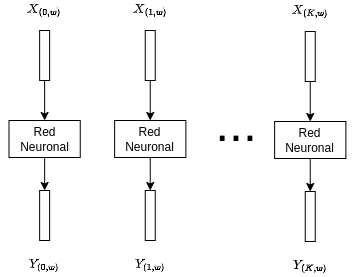
\includegraphics[scale=0.7]{images/ch3/features-ffnn.png}}
	\caption{Procesamiento de espectrogramas con una red del tipo feedforward.}
	\label{fig:ch3_features_ffnn}
\end{figure}

Una forma de procesar, con la red neuronal, la matriz $X(n, w)$, es armar vectores formados por J filas, con la forma $[X(i-J+1,w), X(i-J+2,w), ... , X(i,w)]$. Donde $J$ es la cantidad de ventanas hacia atrás del tiempo $i$ que se utilizan para determinar $Y(i, w)$. 

En la figura \ref{fig:ch3_features_ffnn} podemos ver el proceso para obtener $Y(i, w)$, el cual consta de hacer pasar por la red los vectores $[X(i, w), X(i+1, w), ..., X(i+J-1, w)]$. Por cada vector de entrada, se obtiene, a la salida de la red, el vector $Y(i, w)$. Agrupando todas las salidas finalmente se obtiene $Y(n, w)$.

Uno de los problema de esta solución, es que la dimensión del vector de entrada crece rápidamente a medida que $J$ se hace mas grande. Cada vector $X(i, w)$ tiene un tamaño de $N/2$ muestras, donde $N$ es la cantidad de muestras utilizados en la $DFT$ de $x(m) \omega(nR-m)$. Entonces, por ejemplo, para $N=1024$ y $J=32$, tendríamos un vector de entrada de dimensión $512 \cdot 32 = 16384$. Otro de los problemas con este enfoque, es que la salida $Y(i, w)$, queda como un función de todos los puntos del vector de entrada, algo que esta lejos de representar correctamente las dependencias temporales existentes en las señales de habla.

\subsubsection{Redes neuronales del tipo convolucionales}
\label{sec:redes_convolucionales}

Una de las estructuras de redes neuronales que permite procesar información n-dimensional y aprender características locales, son las redes convolucionales \cite{deep_learning}. 

Las redes convolucionales están formadas por capas convolucionales, las cuales poseen una serie de filtros o \emph{kerneles}. Estos filtros se adaptan durante el entrenamiento de manera tal que se pueda obtener características locales, abarcando las n dimensiones.

A diferencia de las redes \emph{feedforward} donde para procesar la matriz:

\begin{equation*}
	\{X(i, w), X(i+1, w), ..., X(i+J-1, w)\}
\end{equation*}

\noindent es necesario desarmarla y formar un vector. Con la red convolucional, se la puede procesar sin modificación alguna. En la figura \ref{fig:ch3_features_cnn}, podemos ver el proceso para obtener $Y(n, w)$ a partir de $X(n, w)$.

\begin{figure}
	\centering
	\centerline{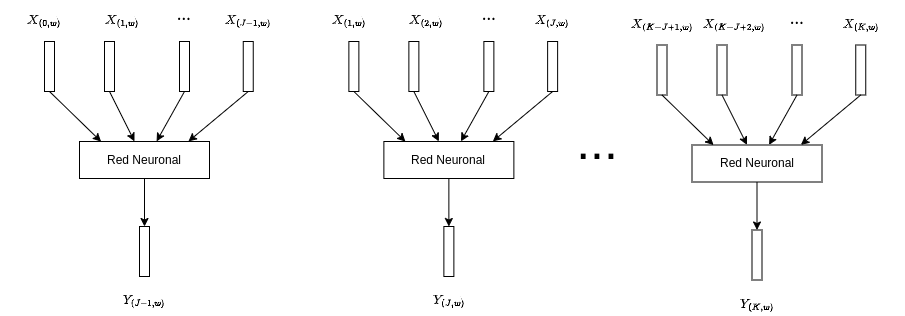
\includegraphics[scale=0.5]{images/ch3/features-cnn.png}}
	\caption{Procesamiento de espectrogramas con una red del tipo convolucional.}
	\label{fig:ch3_features_cnn}
\end{figure}

\subsubsection{Redes neuronales auto-codificadoras}
\label{sec:redes_autocodificadoras}

El diseño de una arquitectura de red neuronal involucra múltiples factores. Uno de ellos es la elección del tipo de capa a utilizar. Como vimos en la sección anterior, algunos de los tipos de capas que se pueden utilizar son las capas feedforward o las capas convolucionales. 

Otro de los factores a diseñar es cómo la arquitectura logrará cumplir el objetivo final, el cual en nuestro caso es el de reducir el ruido en las señales de habla. Una de las arquitecturas de redes que tiene esta característica son las redes auto-codificadoras.

Una red auto-codificadora es un tipo de red entrenada para generar una copia de la entrada \cite{deep_learning}. Como se muestra en la figura \ref{fig:ch3_autoencoder}, la red se puede dividir en dos, una función codificadora $h=f(x)$ y una función decodificadora $r=g(h)$. En conjunto, ambas partes aprenden la identidad $g(f(x)) = x$.

Una de las aplicaciones más comunes es la de utilizarla como una reductora de la dimensión de entrada. Cuando a una red auto-codificadora se la entrena para reducir la dimensión de entrada, se la fuerza a capturar las características más importantes del conjunto de entrenamiento.

\begin{figure}
	\centering
	\centerline{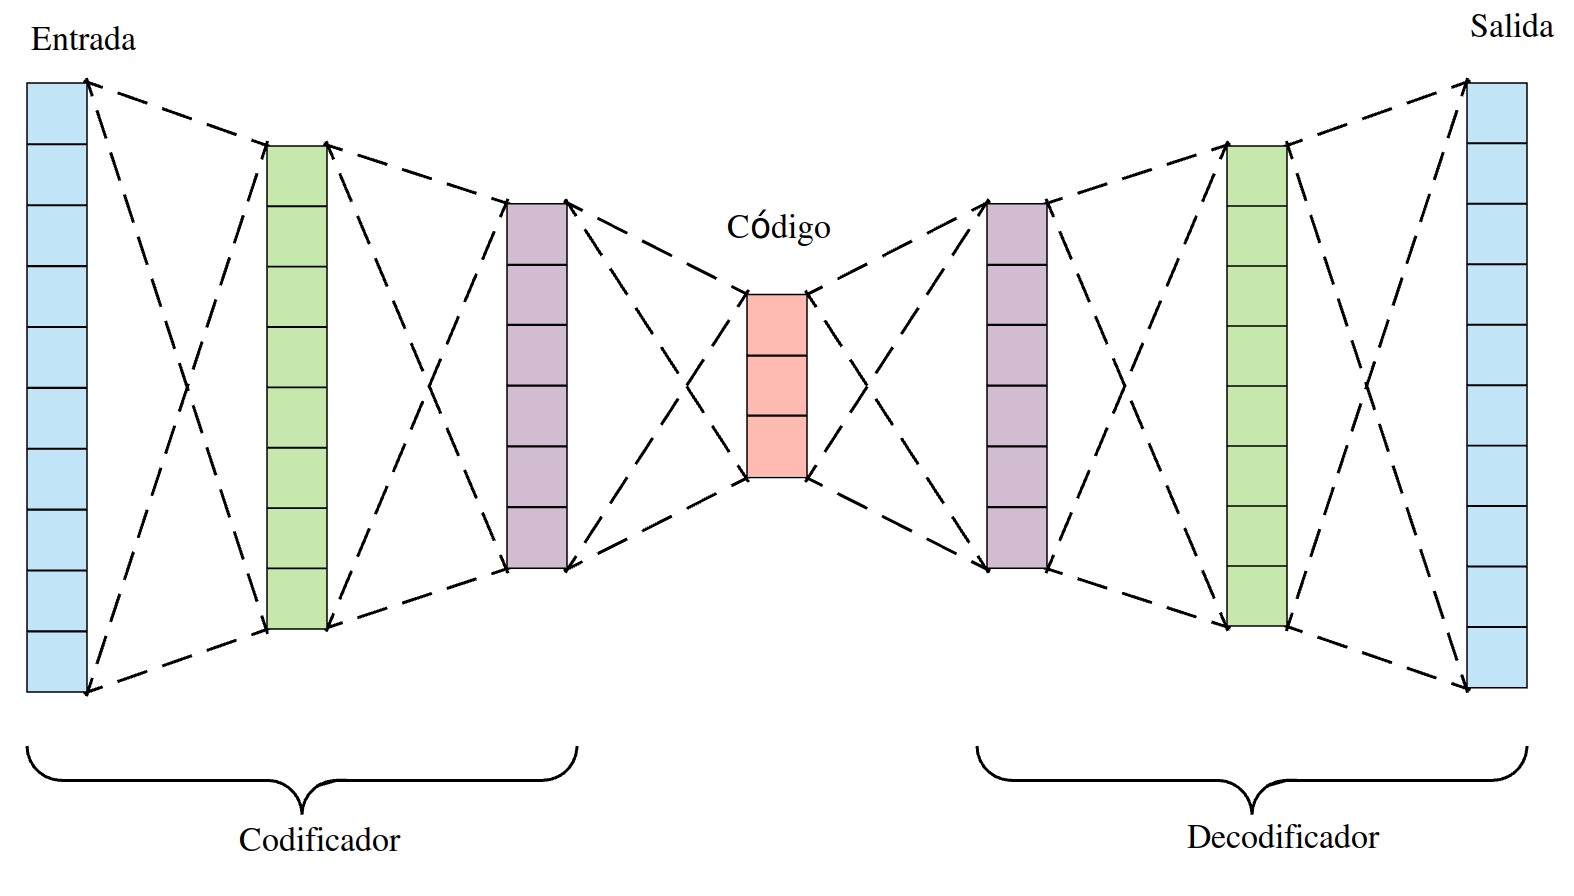
\includegraphics[scale=0.2]{images/ch3/autoencoder.png}}
	\caption{Red neuronal del tipo auto-codificadora.}
	\label{fig:ch3_autoencoder}
\end{figure}

El objetivo del codificador es reducir el tamaño de las señales, de forma tal que al ser decodificadas, la señal resultante minimice cierta función de error respecto de la señal original. Generalmente la función de error utilizada es el error cuadrático medio.

Otra de las funciones comunes de las redes auto-codificadoras es la de remover ruido. A la entrada del codificador se presentan las señales ruidosas y a la salida las señales filtradas. Con esto el auto-codificador aprende a generar la señal filtradas, utilizando la menor cantidad de información posible y por ende aprende a mantener la información relevante de la señal y descartar el ruido.

\subsubsection{Redes neuronales auto-codificadoras con estructura del tipo U}
\label{sec:redes_tipo_u}

La arquitectura del tipo U se usó por primera vez en un trabajo de segmentación de imágenes bio-médicas \cite{U_Net_Convolutional_Networks_for_Biomedical_Image_Segmentation}. En este tipo de tareas la red debe aprender a asignar una etiqueta a cada píxel de la imagen de entrada. Para logarlo, se necesita un modelo de red neuronal capaz de trabajar con gran precisión y localización, es decir trabajar a nivel de un píxel y capaz de localizar áreas con gran exactitud.

Estas características de las redes del tipo U hacen que sean efectivas para trabajar en el dominio de la STFT, donde un desplazamiento en tiempo o en frecuencia afecta considerablemente la calidad y la inteligibilidad de los sonidos. En \cite{singing_voice_separation_with_deep_u_net_convolutional_networks} este tipo de arquitectura fue utilizada para una aplicación de separación de fuentes en señales de audio.

La arquitectura del tipo U consta de un codificador y un decodificador. En la figura \ref{fig:ch3_unet} podemos ver el codificador en los bloques de la izquierda y el decodificador en los bloques de la derecha.

\begin{figure}
	\centering
	\centerline{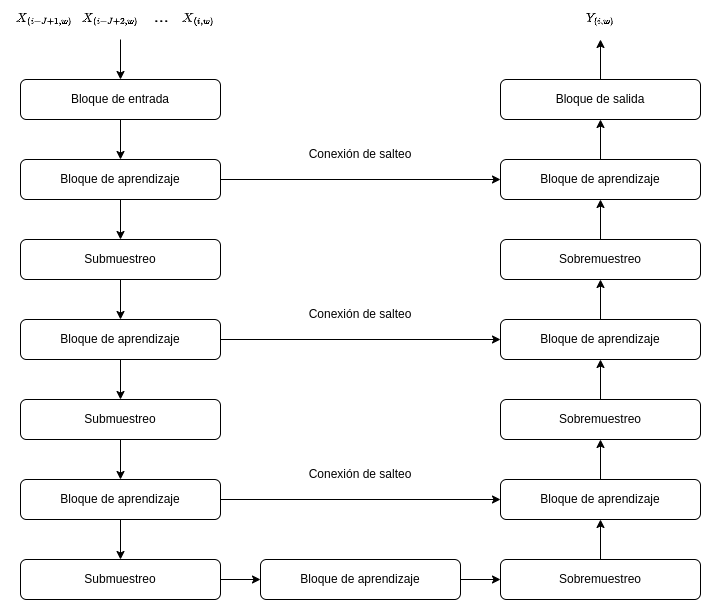
\includegraphics[scale=0.65]{images/ch3/unet.png}}
	\caption{Red neuronal auto-codificadora del tipo U.}
	\label{fig:ch3_unet}
\end{figure}

El codificador de la red consiste en el camino contractivo, el cual se encarga de reducir la dimensión. Esto lo logra por medio de:

\begin{enumerate}
	\item Un bloque de aprendizaje, que se encarga de aprender atributos locales. Estos bloques son esencialmente convolucionales. Aumentan la cantidad de canales de la señal de entrada, permitiendo ajustar los filtros de tal manera que cada nivel aprende a distinguir ciertos rasgos de la señal de entrada.
	
	\item Un bloque de sub-muestreo que reduce a la mitad la dimensión de su entrada. La reducción la logra por medio de la ejecución de operaciones de agrupación por máximo valor (\emph{max pooling} \cite{deep_learning}). La operación de agrupación por máximo valor es esencial para que se mantengan los atributos relevantes y se descarten los restantes.
\end{enumerate}

El decodificador de la red consiste en el camino expansivo. Realiza la tarea opuesta al camino contractivo, es decir, aumenta la dimensión, nuevamente con un bloque de aprendizaje y con un bloque de sobre-muestreo:


\begin{enumerate}
	\item Nuevamente el bloque de aprendizaje se encarga de obtener atributos relevantes. En lugar de aumentar la cantidad de canales de la señal de entrada los reduce, permitiendo recuperar la señal de entrada sin los rasgos indeseables.
	
	\item Un bloque de sobre-muestreo que aumenta al doble la dimensión de su entrada. El aumento lo logra por medio de la ejecución de operaciones de interpolación.
\end{enumerate}

Además, a la salida de los bloques de aprendizaje tenemos una conexión de salteo. Estas conexiones permiten al camino expansivo recuperar características de la señal original. 

Los bloques de aprendizaje del camino expansivo reciben una entrada compuesta por; la salida del bloque anterior junto con la concatenación de la salida del bloque de aprendizaje del camino contractivo. Esto les permite operar con el doble de información \cite{the_importance_of_skip_connections_in_biomedical_image_segmentation}.

Veamos cómo se componen cada uno de los bloques de la figura \ref{fig:ch3_unet}. El bloque de entrada está compuesto por:

\begin{itemize}
	\item Una capa convolucional con un núcleo de tamaño 3x3, un paso de 1 y un rellenado de 1. Esta combinación de parámetros permite obtener una señal de igual tamaño que la utilizada como entrada, resultante de la convolución entre los filtros y la señal de entrada a la capa.
	\item Una función de activación del tipo ReLU \cite{deep_learning}.
	\item Una función de agrupación por máximo valor, que reduce el tamaño en un factor de 2, tanto en frecuencia como en el tiempo.
\end{itemize}

El bloque de aprendizaje está compuesto por:

\begin{itemize}
	\item Una capa de normalización por lote \cite{deep_learning}.
	\item Un capa convolucional con un núcleo de tamaño 3x3 un paso de 1 y un rellenado de 1.
	\item Una función de activación del tipo ReLU.
\end{itemize}

El bloque de sub-muestreo se compone únicamente de una función de agrupación por máximo valor, que reduce el tamaño en 2.

El bloque de sobre-muestreo se compone únicamente de una función de interpolación bilineal que aumenta el tamaño en una factor de 2.

El bloque de salida está compuesto por:

\begin{itemize}
	\item Una función de interpolación bilineal que aumenta el tamaño en un factor de 2.
	\item Un capa convolucional con un núcleo de tamaño 3x3 un paso de 1 y un rellenado de 1.
\end{itemize}

Las capas convolucionales, aumentan por un factor de 2 la cantidad de canales de los espectrogramas en el camino expansivo y lo reducen por un factor de 2 en el camino contractivo. En el bloque intermedio, se mantiene la cantidad de canales a la salida respecto de la entrada.

\subsubsection{Procesamiento de las señales de habla}
\label{sec:filtro_neuronal_procesamiento_de_señales}

A diferencia del caso del filtro adaptativo, donde trabajamos en el dominio del tiempo, en el filtro neuronal trabajamos en el dominio de la STFT. Como vimos en la sección \ref{sec:redes_convolucionales}, la información de entrada de la red son espectrogramas formados por $J$ ventanas de la señal de habla ruidosa $x[n]$.

Cada espectrograma se forma con una ventana deslizante, la cual incluye $J$ sub-ventanas de la señal $x[n]$ de manera que el espectrograma tenga un tamaño en el dominio del tiempo de $J$. La ventana deslizante se mueve de a una sub-ventana a la vez y por cada movimiento se obtiene un nuevo espectrograma que servirá como entrada a la red. Este proceso se muestra en la figura \ref{fig:ch3_procesamiento_señal_habla_entrada}.

\begin{figure}
	\centering
	\centerline{\includegraphics[scale=0.45]{images/ch3/procesamiento_señal_habla_entrada.png}}
	\caption{Ventaneo de la señal de entrada.}
	\label{fig:ch3_procesamiento_señal_habla_entrada}
\end{figure}

Por cada ventana deslizante procesada por la red, se obtiene una ventana de la señal filtrada. Al pasar todas las ventanas deslizantes por la red, se forma a la salida la señal de habla filtrada. Este proceso se muestra en la figura \ref{fig:ch3_procesamiento_señal_habla_salida}.

\begin{figure}[H]
	\centering
	\centerline{\includegraphics[scale=0.45]{images/ch3/procesamiento_señal_habla_salida.png}}
	\caption{Obtención de la señal de habla filtrada.}
	\label{fig:ch3_procesamiento_señal_habla_salida}
\end{figure}

A diferencia del caso del filtro adaptativo, donde la señal filtrada se obtiene de una muestra a la vez, en el filtro neuronal la señal de habla filtrada se obtiene de una ventana a la vez.